\section{Algorithm}
\label{sec:overview}

%\textbf{Problem Definition.}
A multi-camera system is set up to capture objects in an indoor scene, as shown in Fig.~\ref{fig:rig}.
%The cameras in our 3D reconstruction system are placed on the periphery of the room pointing inwards, only the neighboring cameras have overlapping fields of view. \xj{what is the point of this overlapping fov?}
%
$K$ ($K=8$) camera pods are installed around the working space looking inwards for a full capture.
Each camera pod consists of one color camera and two Near Infra-Red (NIR) cameras. A laser pointer is used to produce special patterns.
From a pair of images of the projected patterns captured by the two NIR cameras, a depth map $D_k$ can be estimated using the PatchMatch stereo algorithm~\cite{Bleyer2011PatchMatch}.
There are also several alternative depth cameras or depth estimation algorithm to obtain the depth map of each view. Most of them produce a rough depth map with noise and errors.
As Fig.~\ref{fig:deptherror} shows, the estimated depth map encounters distortions on the boundary of the human body, and missing data in the head area.
How to improve the quality of depth map is beyond the scope of this paper.

\begin{figure}
	\centering
	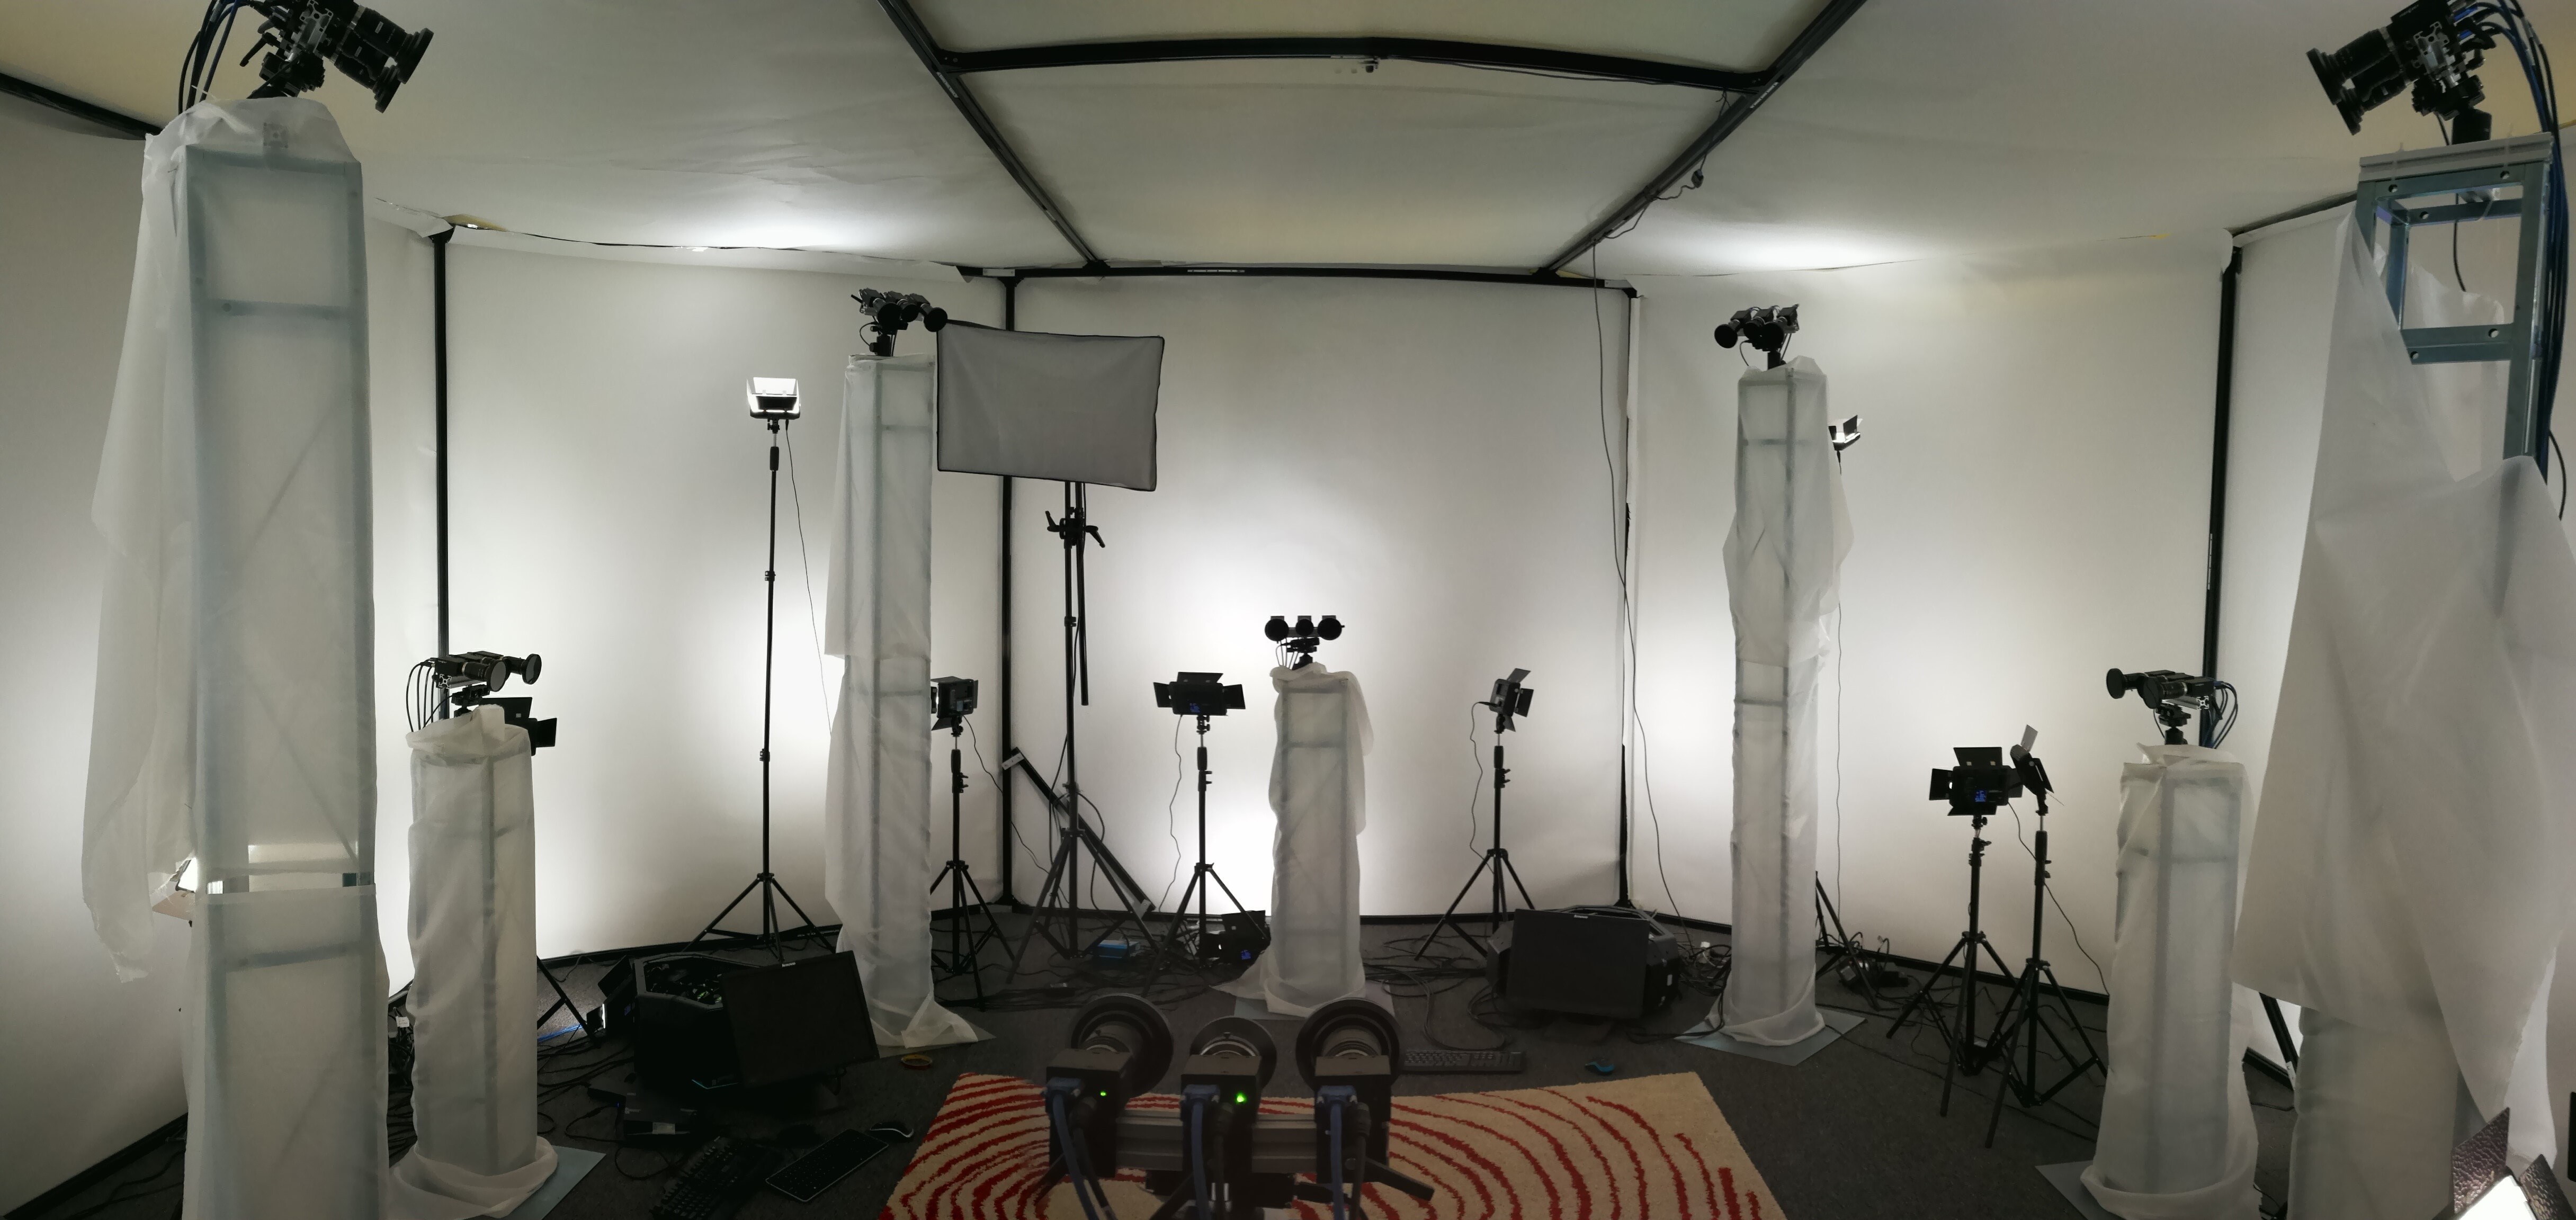
\includegraphics[width=\columnwidth]{image/rig.jpg}
	\caption{Our multi-camera system with 8 camera pods pointing inwards.}
	\label{fig:rig}
\end{figure}



\begin{figure*}[ht]
	\centering
	\subfigure[]{
		\begin{minipage}[c]{.22\linewidth}
			\centering
			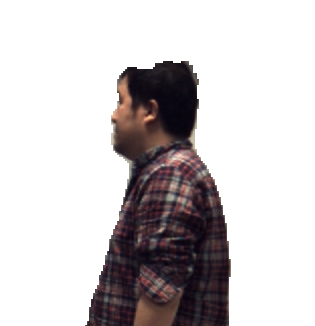
\includegraphics[width=4cm]{image/depth_error_rgb.png}
		\end{minipage}
	}%
	\subfigure[]{
		\begin{minipage}[c]{.22\linewidth}
			\centering
			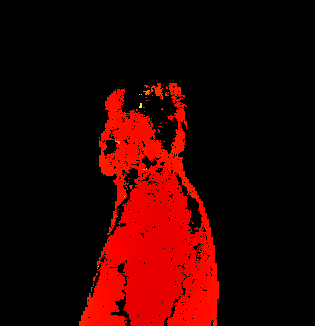
\includegraphics[width=4cm]{image/depth_error_depth2.png}
		\end{minipage}
	}
	\subfigure[]{
		\begin{minipage}[c]{.22\linewidth}
			\centering
			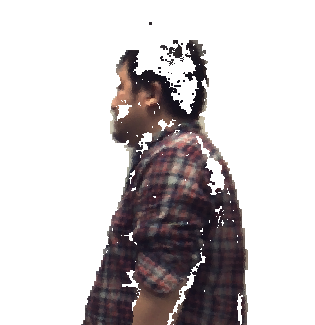
\includegraphics[width=4cm]{image/depth_error_pc.png}
		\end{minipage}
	}
	\subfigure[]{
		\begin{minipage}[c]{.22\linewidth}
			\centering
			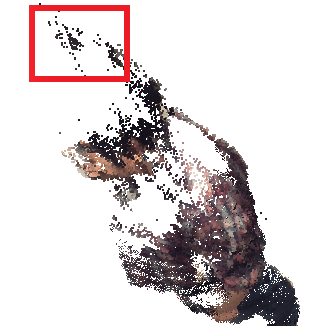
\includegraphics[width=4cm]{image/depth_error_pc_2.png}
		\end{minipage}
	}
	\caption{Errors in depth estimation. (a) RGB; (b) Depth; (c) The point cloud reconstructed from RGBD data. (d) Another view of the point cloud. The distortion of the head region (in the red box) is caused by the inaccurate depth estimation. }
	\label{fig:deptherror}
\end{figure*}



%
Under the pinhole camera assumption, each camera has a group of parameters including the intrinsic matrix $K$ and extrinsic matrix $M$ to project a point in the 3D space to its image plane as
\begin{equation}\label{eq:cam-proj}
z_{p}\mathbf{x}=\mathbf{K}\mathbf{M}\mathbf{p},
\end{equation}
where $\mathbf{p}=(x,y,z,1)^{T}$ is the homogeneous coordinate of the 3D point, and $\mathbf{x}=(u,v,1)^{T}$ is the homogeneous coordinate of its projected point on the image plane.
%


From the depth map estimated by each camera pod, a partial point cloud can be reconstructed by back-projecting each pixel in the depth map into the 3D space according to the parameters of each camera.
%
A 3D model can be obtained by fusing the $K$ point clouds.
%
%
Ideally, with the accurate depth $z_p$ of each image point $\vb{x}$, and accurate camera parameters $\camin$ and $\camex$, the image pixels captured in different views can be back-projected to the 3D space and well aligned in the 3D space.
%
However, due to the unavoidable error and noises in depth maps, the points cloud obtained in different views deviate a lot even with accurate camera poses.
We divide the pipeline into two main parts to reconstruct a high-quality model.
%
The first part is a global camera calibration method to estimate the camera parameters $\{\camin_k, \camex_k\}^{K}_{k=1}$ as accurate as possible, as described in Sec.~\ref{sec:global-calib}.
The second is a registration method to produce 3D point clouds as consistent as possible from in-accurate depth $z_p$, as described in Sec.~\ref{sec:registration}.


\comments{

Our algorithm consists of two main parts. Firstly, we use the toolbox Kalibr~\cite{Maye2013Self} to calibrate our multi-camera system and achieve the intrinsic and initial extrinsic parameters of all our cameras. Then we use a checkerboard as the calibration object, detect the corners on it and do the global extrinsic parameters optimization, as described in Sec.~\ref{sec:global-calib}.
%
Secondly, we use the camera parameters and the input RGB and depth images to reconstruct the point clouds of the model and use ICP (Iterative Closest Point)~\cite{Besl1992A} to align the point clouds of different views.
With the transform of the registration, the error caused by depth estimation can be minimized and a more accurate 3D reconstruction can be achieved, as described in Sec.~\ref{sec:registration}.
Finally, we compare the reconstruction results using different methods. We also compute the reprojection error and use a plaster model as the ground truth to verify the effectivity of our algorithm, as described in Sec.~\ref{sec:Results}.
\xj{Show a system pipeline.}
}

